\section{Proposed Algorithm}\label{sec:method}
\subsection{Whole-Line Plans}
Let $\mathcal X_l$ contain all binary solutions of line $l$ that satisfy \eqref{eq:assign}--\eqref{eq:fatigue} and \eqref{eq:recovery}. The shared limits in \eqref{eq:sharedh} and \eqref{eq:sharedr} remain outside this set. A pricing model can use the redundant bounds $\sum_s h_{ls}\leq k_l$ and $\sum_s r_{ls}\leq k_l$. These bounds do not allocate global resources to a line.

A column $p\in\mathcal P_l$ represents one complete plan in $\mathcal X_l$. It records the selected tasks, their stations and modes, and the associated station configurations. Define
\begin{align}
h_{lp}&=\sum_s h_{ls}^p,&r_{lp}&=\sum_s r_{ls}^p,\label{eq:features}\\
c_{lp}&=\sum_i v_{li}y_{li}^p-\sum_{i,s,m}c_{li}^{m}x_{lism}^p\nonumber\\
&\quad-\sum_s(c_{ls}^{0}u_{ls}^p+c_{ls}^{H}h_{ls}^p+c_{ls}^{R}r_{ls}^p).\label{eq:colprofit}
\end{align}
An empty station is allowed within a plan. A completely empty line plan exists only if the required-task and recovery conditions allow it. Columns with the same selected task set can still differ in station assignment or mode. Deduplication therefore uses the complete assignment pattern.

\begin{figure*}[!tp]\centering
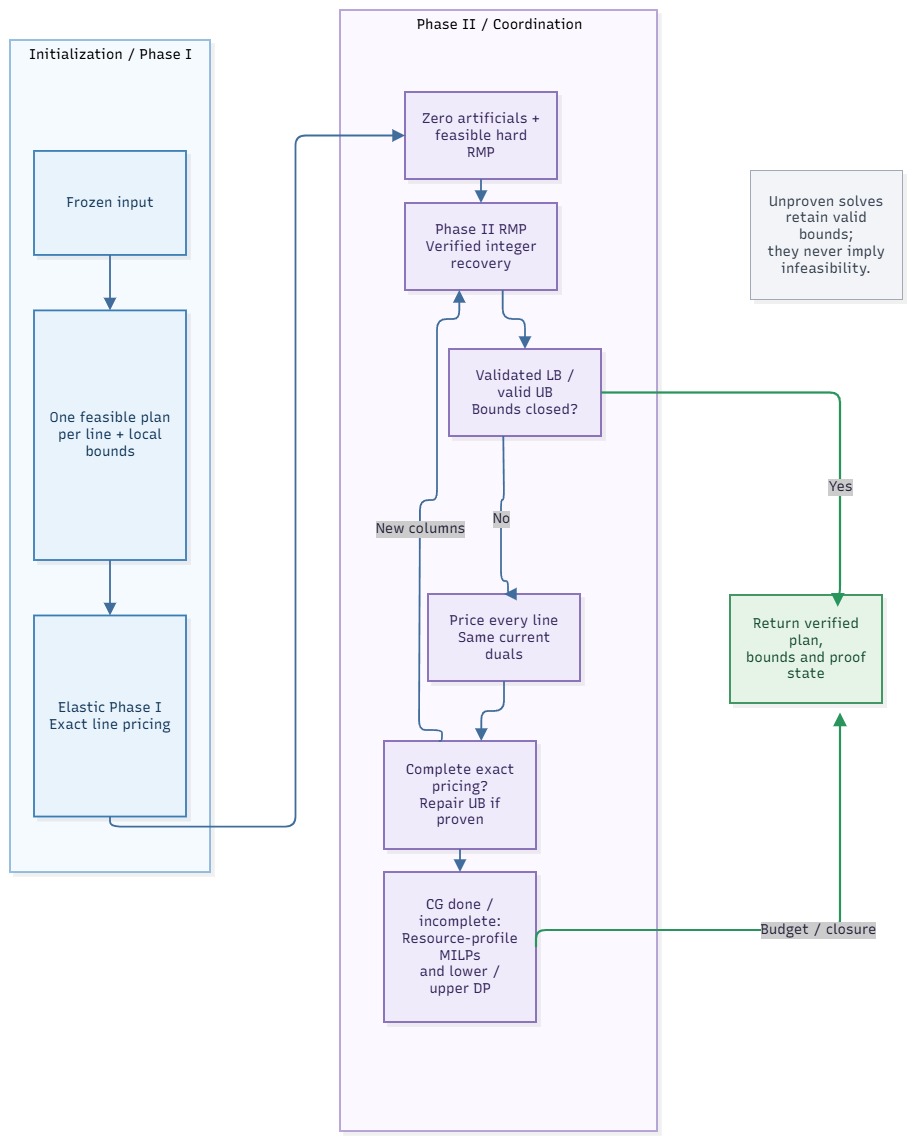
\includegraphics[width=\textwidth,height=0.67\textheight,keepaspectratio]{img/algorithm_flowchart.png}
\caption{Proposed framework. CG coordinates complete line plans; verified integer recovery and resource-profile bounds provide separate integer proof paths. Only complete exact pricing repairs the CG dual bound. A budget stop returns the actual proof state and remaining gap.}\label{fig:flow}
\end{figure*}
Fig.~\ref{fig:flow} shows the solution workflow. A station-level column can be locally feasible but difficult to combine across stations. A whole-line column already satisfies task uniqueness, required-task selection, all precedence prefixes, and line recovery. Integer combination then requires coordination of the two resource totals. The two-phase CG loop supplies LP coordination, while restricted integer recovery and profile queries address the remaining integer gap.

\subsection{Master Problem and Formulation Strength}
Binary $\lambda_{lp}$ selects one plan for line $l$. The complete master problem is
\begin{align}
\max\quad&\sum_l\sum_{p\in\mathcal P_l}c_{lp}\lambda_{lp},\label{eq:master}\\
\text{s.t.}\quad&\sum_{p\in\mathcal P_l}\lambda_{lp}=1&&\forall l,\label{eq:convex}\\
&\sum_{l,p}h_{lp}\lambda_{lp}\leq h^{\max},\label{eq:masterh}\\
&\sum_{l,p}r_{lp}\lambda_{lp}\leq r^{\max},\label{eq:masterr}\\
&\lambda_{lp}\in\{0,1\}.\label{eq:masterbinary}
\end{align}
Column profit already includes all station and resource costs.

\begin{proposition}\label{prop:equiv}
The complete integer master and the compact MILP have the same feasible objective values.
\end{proposition}
\begin{proof}
Extract the binary variables of each line from a feasible compact solution. They form a member of $\mathcal X_l$ and hence a column. Selecting these columns preserves the resource totals and every objective term. Conversely, select one column per line from a feasible integer master solution. Copy its task, station, and mode variables to the compact model. Local feasibility follows from $\mathcal X_l$. Shared feasibility follows from \eqref{eq:masterh} and \eqref{eq:masterr}. The two-way configuration logic fixes activation and deployment, including empty stations. The reconstructed profit is unchanged.
\end{proof}

The complete linear programming (LP) relaxation replaces \eqref{eq:masterbinary} by $\lambda_{lp}\geq0$. Let $z_{\rm line}^{\LP}$, $z_{\rm station}^{\LP}$, and $z_{\rm compact}^{\LP}$ denote the complete line, complete station, and compact LP bounds. Then
\begin{equation}
z^{\IP}\leq z_{\rm line}^{\LP}\leq z_{\rm station}^{\LP}\leq z_{\rm compact}^{\LP}.\label{eq:hierarchy}
\end{equation}
Every line-plan mixture induces station-plan mixtures with identical weights and objective. Station-plan mixtures in turn induce feasible compact fractional assignments. This establishes the inclusions in \eqref{eq:hierarchy}. The supplementary file gives the detailed mapping. These comparisons concern complete column sets, not arbitrary restricted pools.

\subsection{Restricted Master and Exact Pricing}
CG maintains a finite pool $\overline{\mathcal P}_l\subseteq\mathcal P_l$. Its restricted master problem (RMP) uses the LP version of \eqref{eq:master}--\eqref{eq:masterr} over this pool. The dual variables are $\sigma_l\in\mathbb R$ for \eqref{eq:convex} and $\pi_H,\pi_R\geq0$ for the resource rows. The complete dual is
\begin{align}
\min\quad&D=\sum_l\sigma_l+h^{\max}\pi_H+r^{\max}\pi_R,\label{eq:dual}\\
\text{s.t.}\quad&\sigma_l+\pi_Hh_{lp}+\pi_Rr_{lp}\geq c_{lp}&&\forall l,p.
\end{align}
The reduced cost of a column is
\begin{equation}
\bar c_{lp}=c_{lp}-\pi_Hh_{lp}-\pi_Rr_{lp}-\sigma_l.\label{eq:rc}
\end{equation}
Pricing solves one MILP per line:
\begin{equation}
\rho_l=\max_{p\in\mathcal P_l}\{c_{lp}-\pi_Hh_{lp}-\pi_Rr_{lp}-\sigma_l\}.\label{eq:pp}
\end{equation}
The objective increases the effective deployment costs by $\pi_H$ and $\pi_R$. All line constraints remain unchanged. Task coverage and precedence do not have separate master duals in this formulation. They belong to the pricing domain.

A new legal column enters the pool if its independently recomputed reduced cost exceeds $\varepsilon_{rc}$. All lines use the same RMP dual solution in a round. The implementation reuses one native CPLEX model per line. It updates every objective coefficient and submits the previous full integer solution as a warm start. Separate line sessions prevent state contamination.

\subsection{Initialization and Phase I}
A short economic MILP first seeks a feasible plan on each line. A constant-objective solve provides a fallback. A proven empty local domain implies global infeasibility. A time limit without a plan does not establish emptiness.

Local plans can conflict in their combined resource demands. Phase I keeps each convexity equation hard and adds nonnegative elastic variables:
\begin{align}
\max\quad&-a_H-a_R,\label{eq:p1}\\
\text{s.t.}\quad&\sum_p\lambda_{lp}=1&&\forall l,\nonumber\\
&\sum_{l,p}h_{lp}\lambda_{lp}-a_H\leq h^{\max},\nonumber\\
&\sum_{l,p}r_{lp}\lambda_{lp}-a_R\leq r^{\max},\nonumber\\
&\lambda_{lp},a_H,a_R\geq0.\nonumber
\end{align}
One local plan per line makes this elastic RMP feasible. Real columns have zero objective coefficients. The dual satisfies $0\leq\pi_H,\pi_R\leq1$. Phase I pricing maximizes $-\pi_Hh_{lp}-\pi_Rr_{lp}-\sigma_l$ over $\mathcal P_l$.

The complete Phase I optimum is zero exactly when the complete line LP is feasible. A feasible line LP admits zero artificials. Conversely, zero artificials leave all real master constraints satisfied. This equivalence concerns LP feasibility. It does not establish integer feasibility. After the artificial sum reaches its tolerance, the implementation resolves the hard Phase II RMP before proceeding.

\subsection{Valid Bounds and Integer Recovery}
At an optimal RMP solution, repair each convexity dual by $\sigma_l'=\sigma_l+\max(0,\rho_l)$. Complete exact pricing then gives
\begin{equation}
z_{\rm line}^{\LP}\leq u^{CG}=D+\sum_l\max(0,\rho_l).\label{eq:cgub}
\end{equation}
The repaired variables satisfy every complete-dual inequality. This proves the bound by weak duality. When every $\rho_l\leq\varepsilon_{rc}$, the residual LP gap can accumulate across the lines. It is not automatically bounded by one pricing tolerance.

An incomplete or time-limited pricing round does not certify \eqref{eq:cgub}. The implementation still attempts the remaining lines under the same duals. It then stops that CG loop if any pricing maximum remains unproven. Existing valid bounds remain available. A negative complete Phase I repaired bound proves LP infeasibility.

The restricted integer master provides candidate integer plans. A data-level checker and the original compact constraints verify each plan before its profit becomes a lower bound (LB). Restricted integer optimality alone does not imply global integer optimality. Independently, local economic upper bounds $b_l^e\geq\max_{p\in\mathcal P_l}c_{lp}$ give $z^{\IP}\leq z_{\rm line}^{\LP}\leq\sum_l b_l^e$. The implementation also reuses reliable native bounds from full-domain, zero-resource-price economic pricing. It restores the convexity constant before using these bounds. It does not substitute an incumbent for a maximization upper bound (UB).

\subsection{Demand-Driven Resource Profiles}
When the current LB and UB remain separated, define
\begin{equation}
v_l(a,b)=\max\{c_{lp}:p\in\mathcal P_l,\ h_{lp}=a,\ r_{lp}=b\}.\label{eq:profile}
\end{equation}
The integer counts satisfy $a\leq\min(k_l,h^{\max})$ and $b\leq\min(k_l,r^{\max})$. An infeasible profile has value $-\infty$. A profile with no completed solve remains unresolved. Plans with identical resource totals have identical coupling coefficients. Only the most profitable plan of such a profile is needed for integer coordination.

Let $\underline v_l$ contain validated profile incumbents and $\overline v_l$ contain valid profile upper bounds. Unknown upper bounds remain $+\infty$. Prior complete pricing gives
\begin{equation}
\overline v_l(a,b)\leq\sigma_l+\max(0,\rho_l)+\pi_Ha+\pi_Rb.\label{eq:profilecut}
\end{equation}
The right-hand side is a valid candidate bound; the stored value takes the minimum over valid sources. For a profile table $v$, dynamic programming (DP) uses
\begin{equation}
f_l(A,B)=\max_{a\leq A,b\leq B}
\{f_{l-1}(A-a,B-b)+v_l(a,b)\},\label{eq:dp}
\end{equation}
with $f_0(A,B)=0$. The lower table yields a feasible integer combination. The upper table bounds every feasible integer combination. Its bound can be tighter than the complete line LP bound. Closing this integer bound does not certify LP convergence.

The procedure queries an unresolved profile on an upper-DP maximizing path. It chooses the least-attempted profile and uses deterministic line and profile ordering to break ties. A query fixes exact resource counts in a local economic MILP. Its incumbent improves the lower table. Its valid native bound improves the upper table. Its proven infeasibility removes that profile. Query budgets increase geometrically with repeated attempts. The procedure recomputes both DP tables until the budget ends or the bounds close.

\begin{algorithm}[!t]
\caption{Whole-Line CG With Integer Coordination}\label{alg:main}
\begin{algorithmic}[1]
\REQUIRE Line data, shared capacities, time budget, tolerances.
\ENSURE Verified plan, bounds, and proof state.
\STATE Generate one feasible plan per line by local MILP.
\STATE Record reliable local economic bounds.
\STATE Check independent-plan compatibility and bound closure.
\STATE Solve elastic Phase I by CG; retain explicit pricing states.
\STATE Resolve the hard Phase II RMP after zero artificials.
\WHILE{time remains and Phase II remains unresolved}
\STATE Solve the RMP and verify its primal and dual solution.
\STATE Recover and verify a restricted integer solution.
\STATE Stop if the verified LB closes the valid UB.
\STATE Price every line under the current duals.
\STATE Add legal new positive-reduced-cost columns.
\STATE Update the UB only after complete exact pricing.
\STATE Stop CG on an incomplete pricing proof or LP convergence.
\ENDWHILE
\STATE Query unresolved resource profiles through upper-DP paths.
\STATE Update integer bounds and verify the selected plan.
\STATE Return the actual bound, proof state, and termination reason.
\end{algorithmic}
\end{algorithm}

Algorithm~\ref{alg:main} summarizes the implemented framework. Let the best verified integer profit be $\ell$ and the best valid integer upper bound be $u$. Define
\begin{equation}
g_{abs}=u-\ell,\qquad
g_{rel}=\frac{\max(0,u-\ell)}{\max(1,|\ell|)}.\label{eq:gap}
\end{equation}
Missing bounds produce an unknown gap. Integer optimality requires
\begin{equation}
u-\ell\leq\max\{\varepsilon_{abs},\varepsilon_{rel}\max(1,|\ell|)\}.\label{eq:closure}
\end{equation}
A bound below the verified LB beyond the consistency tolerance triggers a numerical error. All proofs use solver floating-point contracts. They are not exact rational certificates. The reported implementation combines root CG and profile DP. Its experiments do not measure a branch-and-price search tree.
